% Options for packages loaded elsewhere
\PassOptionsToPackage{unicode}{hyperref}
\PassOptionsToPackage{hyphens}{url}
\PassOptionsToPackage{dvipsnames,svgnames*,x11names*}{xcolor}
%
\documentclass[
  10pt,
  english,
]{article}
\usepackage{lmodern}
\usepackage{amssymb,amsmath}
\usepackage{ifxetex,ifluatex}
\ifnum 0\ifxetex 1\fi\ifluatex 1\fi=0 % if pdftex
  \usepackage[T1]{fontenc}
  \usepackage[utf8]{inputenc}
  \usepackage{textcomp} % provide euro and other symbols
\else % if luatex or xetex
  \usepackage{unicode-math}
  \defaultfontfeatures{Scale=MatchLowercase}
  \defaultfontfeatures[\rmfamily]{Ligatures=TeX,Scale=1}
\fi
% Use upquote if available, for straight quotes in verbatim environments
\IfFileExists{upquote.sty}{\usepackage{upquote}}{}
\IfFileExists{microtype.sty}{% use microtype if available
  \usepackage[]{microtype}
  \UseMicrotypeSet[protrusion]{basicmath} % disable protrusion for tt fonts
}{}
\makeatletter
\@ifundefined{KOMAClassName}{% if non-KOMA class
  \IfFileExists{parskip.sty}{%
    \usepackage{parskip}
  }{% else
    \setlength{\parindent}{0pt}
    \setlength{\parskip}{6pt plus 2pt minus 1pt}}
}{% if KOMA class
  \KOMAoptions{parskip=half}}
\makeatother
\usepackage{xcolor}
\IfFileExists{xurl.sty}{\usepackage{xurl}}{} % add URL line breaks if available
\IfFileExists{bookmark.sty}{\usepackage{bookmark}}{\usepackage{hyperref}}
\hypersetup{
  pdftitle={Vision-language-action policies versus world models for robot learning},
  pdflang={en},
  colorlinks=true,
  linkcolor=blue,
  filecolor=Maroon,
  citecolor=Blue,
  urlcolor=blue,
  pdfcreator={LaTeX via pandoc}}
\urlstyle{same} % disable monospaced font for URLs
\usepackage[margin=2.2cm]{geometry}
\usepackage{longtable,booktabs}
% Correct order of tables after \paragraph or \subparagraph
\usepackage{etoolbox}
\makeatletter
\patchcmd\longtable{\par}{\if@noskipsec\mbox{}\fi\par}{}{}
\makeatother
% Allow footnotes in longtable head/foot
\IfFileExists{footnotehyper.sty}{\usepackage{footnotehyper}}{\usepackage{footnote}}
\makesavenoteenv{longtable}
\usepackage{graphicx}
\makeatletter
\def\maxwidth{\ifdim\Gin@nat@width>\linewidth\linewidth\else\Gin@nat@width\fi}
\def\maxheight{\ifdim\Gin@nat@height>\textheight\textheight\else\Gin@nat@height\fi}
\makeatother
% Scale images if necessary, so that they will not overflow the page
% margins by default, and it is still possible to overwrite the defaults
% using explicit options in \includegraphics[width, height, ...]{}
\setkeys{Gin}{width=\maxwidth,height=\maxheight,keepaspectratio}
% Set default figure placement to htbp
\makeatletter
\def\fps@figure{htbp}
\makeatother
\setlength{\emergencystretch}{3em} % prevent overfull lines
\providecommand{\tightlist}{%
  \setlength{\itemsep}{0pt}\setlength{\parskip}{0pt}}
\setcounter{secnumdepth}{-\maxdimen} % remove section numbering
\ifxetex
  % Load polyglossia as late as possible: uses bidi with RTL langages (e.g. Hebrew, Arabic)
  \usepackage{polyglossia}
  \setmainlanguage[]{english}
\else
  \usepackage[shorthands=off,main=english]{babel}
\fi
\usepackage[]{natbib}
\bibliographystyle{plainnat}

\title{Vision-language-action policies versus world models for robot
learning}
\usepackage{etoolbox}
\makeatletter
\providecommand{\subtitle}[1]{% add subtitle to \maketitle
  \apptocmd{\@title}{\par {\large #1 \par}}{}{}
}
\makeatother
\subtitle{What each family predicts, how the prediction reaches the
actuator, and how far the evidence actually goes}
\author{}
\date{2026-10-19}

\begin{document}
\maketitle

\hypertarget{short-answer-for-a-group-entering-the-field}{%
\subsection{1. Short answer for a group entering the
field}\label{short-answer-for-a-group-entering-the-field}}

Both families are trained on robot trajectories with supervised or
self-supervised objectives; the difference that matters is \emph{what
the target is} and \emph{when the target is consumed}. A
vision-language-action (VLA) policy predicts actions: the observation
and an instruction go in, a chunk of low-level commands comes out, and
the chunk is executed immediately. A world model predicts future
observations (pixels, latents, or a reward), and that prediction is used
in one of three ways: inside the control loop, as the thing being
optimised; offline, to manufacture extra training data for a
conventional policy; or inside a learned environment, where a policy is
trained by reinforcement on imagined rollouts.

If the practical question is ``which gives me a working manipulator
soonest'', the published record currently favours the first family:
VLA-style policies are the systems that have been exercised on real
hardware at several institutions, with blind or randomised evaluation
protocols. World models have the more interesting scientific question
and, so far, the narrower evidence: most claims of large gains are
single-site, and several are measured in simulation or in games. This
report tries to make that asymmetry visible rather than to declare a
winner.

Two cautions frame everything below. First, a predicted video that looks
plausible is not a control result: pixel fidelity and closed-loop task
success are different quantities, and one does not imply the other.
Second, the numbers in the cited papers are produced by different data,
embodiments, task sets and evaluation protocols, and are reported here
as the authors' own claims under their own conditions, not as points on
a common scale.

\hypertarget{scope-dates-and-evidence-base}{%
\subsection{2. Scope, dates and evidence
base}\label{scope-dates-and-evidence-base}}

This is a small, opportunistically assembled corpus, not a systematic
review. Sixteen unique papers are cited. Their centre of mass is
2024--2025: OpenVLA, pi-0, DINO-WM \citep{openvla, pi0, dino_wm} and the
LIBERO benchmark \citep{libero} form the 2023--2024 layer; SmolVLA,
GR00T N1, Gemini Robotics 1.5, WorldVLA, V-JEPA 2, DreamGen, Cosmos,
Dreamer 4, RoboArena and the large behaviour-model study
\citep{smolvla, groot_n1, gemini_robotics15, worldvla, vjepa2, dreamgen, cosmos, dreamer4, roboarena, lbm}
supply the 2025 layer.

The 2026 layer is thin and must be labelled as such. Exactly two 2026
items are discussed: World-Gymnast, which we read as a complete text,
and PlayWorld, for which a full-text HTML acquisition is retained in our
evidence bundle but from which this report used only abstract-level
statements, so it is described strictly at that level
\citep{world_gymnast, playworld}. A search cutoff of 19 October 2026
therefore does \emph{not} mean complete coverage of 2026; it means that
the 2026 slice of this corpus is two papers. Whenever this report says
that something was ``not located'', the claim is about these sixteen
papers only. It is not a statement that no such result exists in the
literature.

What was actually done, and what was not: sources were acquired as HTML
or PDF full text where available, and claims about them are checked
against those texts rather than against abstracts. Nothing was
re-implemented, no benchmark was re-run, and no new measurement was
made. All numbers below are the papers' own, quoted with their
conditions. Coverage of individual papers is uneven and is stated where
it matters: for a few items only metadata or abstract-level text was
used, and at least one of those (PlayWorld) was in fact acquired as a
substantial full-text HTML bundle that this report did not read for its
body.

\hypertarget{the-two-axes-that-actually-separate-the-families}{%
\subsection{3. The two axes that actually separate the
families}\label{the-two-axes-that-actually-separate-the-families}}

Discussions of ``VLA versus world model'' usually blur two independent
choices. The first is what the network is trained to output: actions,
future observations, or both. The second is where that output is
consumed: in the control loop, as training data, or as a training
environment. Table 1 arranges the families along those two axes. Figure
1 draws the same information as data flow.

A third axis, cost, follows from the second. Direct action policies pay
once per executed chunk: a single forward pass, or a short fixed number
of denoising steps for a flow-matching head, followed by open-loop
execution for a few steps. Planning with a world model pays per
candidate sequence, because the model must be rolled forward for each
sample and usually for several refinement iterations. This is the
dominant practical difference between the families at deployment time,
and it is independent of how good either model is.

\begin{longtable}[]{@{}lllll@{}}
\toprule
\begin{minipage}[b]{0.17\columnwidth}\raggedright
Family\strut
\end{minipage} & \begin{minipage}[b]{0.17\columnwidth}\raggedright
Trained to predict\strut
\end{minipage} & \begin{minipage}[b]{0.17\columnwidth}\raggedright
How prediction is used\strut
\end{minipage} & \begin{minipage}[b]{0.17\columnwidth}\raggedright
Supervision that carries the load\strut
\end{minipage} & \begin{minipage}[b]{0.17\columnwidth}\raggedright
Typical inference cost\strut
\end{minipage}\tabularnewline
\midrule
\endhead
\begin{minipage}[t]{0.17\columnwidth}\raggedright
A. Direct action policy (VLA)\strut
\end{minipage} & \begin{minipage}[t]{0.17\columnwidth}\raggedright
action chunk\strut
\end{minipage} & \begin{minipage}[t]{0.17\columnwidth}\raggedright
executed as the controller\strut
\end{minipage} & \begin{minipage}[t]{0.17\columnwidth}\raggedright
action labels from teleoperation or mixed robot data\strut
\end{minipage} & \begin{minipage}[t]{0.17\columnwidth}\raggedright
one pass per chunk, or a few denoising steps for a flow head\strut
\end{minipage}\tabularnewline
\begin{minipage}[t]{0.17\columnwidth}\raggedright
B. Action model with auxiliary future\strut
\end{minipage} & \begin{minipage}[t]{0.17\columnwidth}\raggedright
actions \textbf{and} future frames\strut
\end{minipage} & \begin{minipage}[t]{0.17\columnwidth}\raggedright
actions executed; frames are an auxiliary target\strut
\end{minipage} & \begin{minipage}[t]{0.17\columnwidth}\raggedright
actions plus video, jointly\strut
\end{minipage} & \begin{minipage}[t]{0.17\columnwidth}\raggedright
one pass per chunk for autoregressive heads\strut
\end{minipage}\tabularnewline
\begin{minipage}[t]{0.17\columnwidth}\raggedright
C. World model as planner\strut
\end{minipage} & \begin{minipage}[t]{0.17\columnwidth}\raggedright
future latent or frames under candidate actions\strut
\end{minipage} & \begin{minipage}[t]{0.17\columnwidth}\raggedright
optimised online (sampling, gradient or RL) then executed\strut
\end{minipage} & \begin{minipage}[t]{0.17\columnwidth}\raggedright
action-conditioned video, sometimes action-free\strut
\end{minipage} & \begin{minipage}[t]{0.17\columnwidth}\raggedright
many rollouts per control step\strut
\end{minipage}\tabularnewline
\begin{minipage}[t]{0.17\columnwidth}\raggedright
D. World model as data or trainer\strut
\end{minipage} & \begin{minipage}[t]{0.17\columnwidth}\raggedright
future frames, or reward and value inside imagination\strut
\end{minipage} & \begin{minipage}[t]{0.17\columnwidth}\raggedright
offline: pseudo-labels, data augmentation, or RL inside the model\strut
\end{minipage} & \begin{minipage}[t]{0.17\columnwidth}\raggedright
video plus inverse-dynamics or reward labels\strut
\end{minipage} & \begin{minipage}[t]{0.17\columnwidth}\raggedright
zero at deployment for D1; amortised for D2\strut
\end{minipage}\tabularnewline
\bottomrule
\end{longtable}

Table 1. Four families on the two axes that matter. The rows describe
the dominant pattern of each family, not every implementation: within
family A, for instance, pi-0 uses an iterative flow-matching head rather
than a single regression pass, and re-planning frequency varies by
system \citep{pi0}.

\hypertarget{family-a-policies-that-predict-actions-and-nothing-else}{%
\subsection{4. Family A: policies that predict actions and nothing
else}\label{family-a-policies-that-predict-actions-and-nothing-else}}

OpenVLA is the cleanest reference point: a 7B-parameter vision-language
model fine-tuned to emit discretised action tokens, trained on roughly
970k robot episodes drawn from the Open X-Embodiment mixture, and
evaluated on a Franka arm across a set of language-conditioned
manipulation tasks \citep{openvla}. pi-0 replaces the discrete decoder
with a flow-matching action expert attached to a pretrained VLM and
reports training on the order of 10,000 hours of robot data spanning
seven robot configurations and 68 tasks, with control at up to 50 Hz
\citep{pi0}. SmolVLA pushes the other way: a 450M-parameter policy
trained on 481 community datasets (about 22.9k episodes and 10.6M
frames), designed to train on a single GPU and to run asynchronous
inference on consumer hardware \citep{smolvla}. GR00T N1 is a
dual-system design in which a vision-language component supplies the
slower reasoning and a diffusion-transformer component emits the action
chunk, trained on a data pyramid that mixes web video, synthetic and
real robot data, with a humanoid target \citep{groot_n1}. Gemini
Robotics 1.5 adds an explicit ``think before acting'' stage and reports
transferring motion between embodiments \citep{gemini_robotics15}.

The common property is that no future observation is ever a training
target. Every gradient comes from an action or from the language
grounding that supports it. This is why the family is cheap to deploy
and why it inherits the weaknesses of behaviour cloning: distribution
shift at test time is unmodelled, and a chunk executed open-loop cannot
notice that the world has diverged from the states in the training set.

The evidence for this family is the strongest in the corpus, but it is
uneven in a specific way. Single-site real robot results are routine.
Multi-institution evaluation is rare, and the one systematic instance
here is RoboArena, which distributes pairwise comparisons of generalist
policies over a shared robot pool and reports that rankings stabilise
after roughly a hundred pairwise comparisons \citep{roboarena}. The most
informative single study is the large behaviour-model examination, which
ran about 1,800 blind rollouts across many tasks on a bimanual platform
after training on roughly 1,700 hours of data, and reports
data-efficiency advantages for large behaviour models over smaller
baselines \citep{lbm}. Those are the results that make the family
credible; they are also, deliberately, results about \emph{one} platform
family and one evaluation protocol.

\hypertarget{family-b-action-models-with-auxiliary-future-prediction}{%
\subsection{5. Family B: action models with auxiliary future
prediction}\label{family-b-action-models-with-auxiliary-future-prediction}}

WorldVLA sits between the families: a single autoregressive transformer
over interleaved action and image tokens, trained so that the same model
both predicts the next action and predicts the next frame
\citep{worldvla}. The authors report an improvement of about 4\% on
LIBERO task suites over comparable action-only baselines, together with
a reported 10\% improvement in video-generation FVD; in their analysis
the auxiliary image objective acts as a regulariser that stabilises the
action objective. Crucially, only the action tokens reach the robot. The
predicted frames are a co-training signal, not a plan.

This family is worth understanding because it isolates the value of
prediction with everything else held fixed: the architecture, data and
evaluation stay close to family A, and only the auxiliary target
changes. The honest reading of the reported gains is that they are
modest and measured largely in simulation, and that the benefit is
described by the authors themselves as a training-time effect rather
than a planning capability. A reader who wants to test ``does predicting
the future help control'' cheaply will find this the most tractable
experiment in the whole area, because the baseline is the same model
minus one loss term.

\hypertarget{family-c-world-models-that-plan}{%
\subsection{6. Family C: world models that
plan}\label{family-c-world-models-that-plan}}

Here the prediction is the controller. DINO-WM builds its world model on
frozen DINOv2 features rather than on pixels, trains it on offline play
data, and plans by rolling the latent model forward under sampled action
sequences and scoring them against a goal image \citep{dino_wm}. The
paper reports zero-shot planning across six environments, including
manipulation and navigation, and argues that pre-trained visual features
make the dynamics model learnable from modest data. V-JEPA 2-AC takes
the same latent-prediction philosophy at larger scale: a
video-pretrained encoder, a small action-conditioned predictor trained
on under 62 hours of unlabelled DROID interaction video, and
goal-conditioned planning by cross-entropy-method search in latent
space, with real-robot pick-and-place demonstrations on two robot
platforms in two laboratories \citep{vjepa2}.

Two properties deserve emphasis. First, latent-space models avoid the
trap of judging a plan by how realistic its rendered future looks,
because nothing is rendered. Second, planning cost is real: every
candidate sequence requires a rollout, so these systems are usually
slower per control step than a direct policy and their reported success
rates should be read with that budget in mind. Neither of the two papers
reports a controlled comparison against a well-tuned behaviour-cloning
baseline trained on the same data, which is exactly the comparison a
newcomer would want.

\hypertarget{family-d-world-models-as-data-factories-and-as-training-environments}{%
\subsection{7. Family D: world models as data factories and as training
environments}\label{family-d-world-models-as-data-factories-and-as-training-environments}}

The offline uses are where world models have most clearly changed
practice, because they attack the cost of robot data rather than the
cost of inference.

\emph{Data generation (D1).} DreamGen trains an action-conditioned video
model on robot and general video, then labels the synthetic futures with
an inverse-dynamics model to recover actions, producing demonstration
data for new behaviours. The authors report scaling a single-task policy
to 22 behaviours on a humanoid, and introduce a benchmark for evaluating
generated robot video \citep{dreamgen}. Cosmos supplies the
general-purpose video world-model platform with open weights that this
style of work builds on, though its published evidence is about
generation quality and physical plausibility rather than downstream
control \citep{cosmos}. PlayWorld, in the 2026 slice, argues from
unsupervised play data that diverse contact-rich experience can be
collected without task labels; this report used only its abstract-level
claims, so it is not counted as control evidence here \citep{playworld}.
A substantial full-text HTML acquisition of that paper is retained in
our evidence bundle, but it was acquired rather than read for the body
of this report, so no claims here rest on its full text.

\emph{Training inside the model (D2).} Dreamer 4 trains a policy
entirely inside a learned world model, using imagined rollouts for
reinforcement learning, and reports solving Minecraft from offline data
without environment interaction \citep{dreamer4}. World-Gymnast applies
the recipe to a real arm: a world model pretrained on large-scale robot
video, then policy improvement by reinforcement learning inside the
model, evaluated on a physical arm on 22 tasks. The reported comparison
in that paper is 34\% against 58\% for the same policy trained with
direct real-world reinforcement learning, and a 28.5\% figure in unseen
rooms; the authors present these as evidence that the model-based route
is cheaper per unit of real interaction rather than uniformly better
\citep{world_gymnast}.

The central methodological hazard of this family is model exploitation:
an optimiser that is allowed to search inside a learned model will find
the model's errors, and an imagined success says nothing about the
physical system. Papers in this family are aware of it and usually
report real-robot confirmation, but the confirmation is typically
small-sample and usually single-site, with the two-laboratory, two-arm
planner demonstration of V-JEPA 2 the main exception in this corpus
\citep{vjepa2}. The second hazard is evaluation leakage: if the world
model was pretrained on video that includes the test environment, an
apparent generalisation result may be a retrieval result. Only the
papers that explicitly hold out environments, as World-Gymnast does for
its unseen-room number, give a reader any grip on this.

\hypertarget{data-embodiments-and-compute-the-requirements-are-not-symmetric}{%
\subsection{8. Data, embodiments and compute: the requirements are not
symmetric}\label{data-embodiments-and-compute-the-requirements-are-not-symmetric}}

Table 2 summarises what each system needs. The asymmetry is stark. A
competitive direct policy needs action-labelled robot data, which is
expensive but well understood, and a fine-tuning recipe on a single GPU
is now realistic at the small end: SmolVLA is explicitly designed for
that budget \citep{smolvla}. A world-model planner needs
action-conditioned video of the same embodiment, which is harder to
obtain than action labels in the open-source ecosystem, or a
sufficiently good latent space that action-free video suffices
\citep{dino_wm, vjepa2}. A world-model trainer needs all of that plus a
reward or value signal, plus enough real-robot budget to validate that
imagined improvement transfers \citep{dreamer4, world_gymnast}.

\begin{longtable}[]{@{}lllll@{}}
\toprule
\begin{minipage}[b]{0.17\columnwidth}\raggedright
System\strut
\end{minipage} & \begin{minipage}[b]{0.17\columnwidth}\raggedright
Prediction target\strut
\end{minipage} & \begin{minipage}[b]{0.17\columnwidth}\raggedright
Data reported by the authors\strut
\end{minipage} & \begin{minipage}[b]{0.17\columnwidth}\raggedright
Embodiment\strut
\end{minipage} & \begin{minipage}[b]{0.17\columnwidth}\raggedright
Code / artefacts\strut
\end{minipage}\tabularnewline
\midrule
\endhead
\begin{minipage}[t]{0.17\columnwidth}\raggedright
OpenVLA \citep{openvla}\strut
\end{minipage} & \begin{minipage}[t]{0.17\columnwidth}\raggedright
discretised actions\strut
\end{minipage} & \begin{minipage}[t]{0.17\columnwidth}\raggedright
\textasciitilde970k episodes, Open X-Embodiment\strut
\end{minipage} & \begin{minipage}[t]{0.17\columnwidth}\raggedright
single Franka arm\strut
\end{minipage} & \begin{minipage}[t]{0.17\columnwidth}\raggedright
open weights and fine-tuning code\strut
\end{minipage}\tabularnewline
\begin{minipage}[t]{0.17\columnwidth}\raggedright
pi-0 \citep{pi0}\strut
\end{minipage} & \begin{minipage}[t]{0.17\columnwidth}\raggedright
action chunk (flow)\strut
\end{minipage} & \begin{minipage}[t]{0.17\columnwidth}\raggedright
\textasciitilde10k hours, 7 configurations, 68 tasks\strut
\end{minipage} & \begin{minipage}[t]{0.17\columnwidth}\raggedright
several mobile and static manipulators\strut
\end{minipage} & \begin{minipage}[t]{0.17\columnwidth}\raggedright
weights released; training recipe partial\strut
\end{minipage}\tabularnewline
\begin{minipage}[t]{0.17\columnwidth}\raggedright
SmolVLA \citep{smolvla}\strut
\end{minipage} & \begin{minipage}[t]{0.17\columnwidth}\raggedright
action chunk\strut
\end{minipage} & \begin{minipage}[t]{0.17\columnwidth}\raggedright
481 datasets, \textasciitilde22.9k episodes, 10.6M frames\strut
\end{minipage} & \begin{minipage}[t]{0.17\columnwidth}\raggedright
6-DoF arms, community hardware\strut
\end{minipage} & \begin{minipage}[t]{0.17\columnwidth}\raggedright
code and weights, single-GPU training\strut
\end{minipage}\tabularnewline
\begin{minipage}[t]{0.17\columnwidth}\raggedright
GR00T N1 \citep{groot_n1}\strut
\end{minipage} & \begin{minipage}[t]{0.17\columnwidth}\raggedright
action chunk (diffusion)\strut
\end{minipage} & \begin{minipage}[t]{0.17\columnwidth}\raggedright
data pyramid: web video, synthetic, real\strut
\end{minipage} & \begin{minipage}[t]{0.17\columnwidth}\raggedright
humanoid\strut
\end{minipage} & \begin{minipage}[t]{0.17\columnwidth}\raggedright
open weights and evaluation harness\strut
\end{minipage}\tabularnewline
\begin{minipage}[t]{0.17\columnwidth}\raggedright
Gemini Robotics 1.5 \citep{gemini_robotics15}\strut
\end{minipage} & \begin{minipage}[t]{0.17\columnwidth}\raggedright
action plus embodied reasoning\strut
\end{minipage} & \begin{minipage}[t]{0.17\columnwidth}\raggedright
not disclosed in the paper\strut
\end{minipage} & \begin{minipage}[t]{0.17\columnwidth}\raggedright
several (motion transfer)\strut
\end{minipage} & \begin{minipage}[t]{0.17\columnwidth}\raggedright
not released\strut
\end{minipage}\tabularnewline
\begin{minipage}[t]{0.17\columnwidth}\raggedright
WorldVLA \citep{worldvla}\strut
\end{minipage} & \begin{minipage}[t]{0.17\columnwidth}\raggedright
actions and next frame\strut
\end{minipage} & \begin{minipage}[t]{0.17\columnwidth}\raggedright
LIBERO demonstrations\strut
\end{minipage} & \begin{minipage}[t]{0.17\columnwidth}\raggedright
simulated arm\strut
\end{minipage} & \begin{minipage}[t]{0.17\columnwidth}\raggedright
research code announced\strut
\end{minipage}\tabularnewline
\begin{minipage}[t]{0.17\columnwidth}\raggedright
DINO-WM \citep{dino_wm}\strut
\end{minipage} & \begin{minipage}[t]{0.17\columnwidth}\raggedright
latent future\strut
\end{minipage} & \begin{minipage}[t]{0.17\columnwidth}\raggedright
offline play data per environment\strut
\end{minipage} & \begin{minipage}[t]{0.17\columnwidth}\raggedright
simulated and real arms\strut
\end{minipage} & \begin{minipage}[t]{0.17\columnwidth}\raggedright
code released\strut
\end{minipage}\tabularnewline
\begin{minipage}[t]{0.17\columnwidth}\raggedright
V-JEPA 2-AC \citep{vjepa2}\strut
\end{minipage} & \begin{minipage}[t]{0.17\columnwidth}\raggedright
latent future\strut
\end{minipage} & \begin{minipage}[t]{0.17\columnwidth}\raggedright
\textless62 h unlabelled DROID video for the action module\strut
\end{minipage} & \begin{minipage}[t]{0.17\columnwidth}\raggedright
two Franka setups, two labs\strut
\end{minipage} & \begin{minipage}[t]{0.17\columnwidth}\raggedright
weights and code released\strut
\end{minipage}\tabularnewline
\begin{minipage}[t]{0.17\columnwidth}\raggedright
DreamGen \citep{dreamgen}\strut
\end{minipage} & \begin{minipage}[t]{0.17\columnwidth}\raggedright
video futures plus IDM actions\strut
\end{minipage} & \begin{minipage}[t]{0.17\columnwidth}\raggedright
robot video plus general video\strut
\end{minipage} & \begin{minipage}[t]{0.17\columnwidth}\raggedright
humanoid\strut
\end{minipage} & \begin{minipage}[t]{0.17\columnwidth}\raggedright
model and benchmark described\strut
\end{minipage}\tabularnewline
\begin{minipage}[t]{0.17\columnwidth}\raggedright
Cosmos \citep{cosmos}\strut
\end{minipage} & \begin{minipage}[t]{0.17\columnwidth}\raggedright
video\strut
\end{minipage} & \begin{minipage}[t]{0.17\columnwidth}\raggedright
large video corpora\strut
\end{minipage} & \begin{minipage}[t]{0.17\columnwidth}\raggedright
none (platform)\strut
\end{minipage} & \begin{minipage}[t]{0.17\columnwidth}\raggedright
open weights, permissive licence\strut
\end{minipage}\tabularnewline
\begin{minipage}[t]{0.17\columnwidth}\raggedright
Dreamer 4 \citep{dreamer4}\strut
\end{minipage} & \begin{minipage}[t]{0.17\columnwidth}\raggedright
latent state, reward, value\strut
\end{minipage} & \begin{minipage}[t]{0.17\columnwidth}\raggedright
offline Minecraft data\strut
\end{minipage} & \begin{minipage}[t]{0.17\columnwidth}\raggedright
game agent\strut
\end{minipage} & \begin{minipage}[t]{0.17\columnwidth}\raggedright
code released\strut
\end{minipage}\tabularnewline
\begin{minipage}[t]{0.17\columnwidth}\raggedright
World-Gymnast \citep{world_gymnast}\strut
\end{minipage} & \begin{minipage}[t]{0.17\columnwidth}\raggedright
latent future plus value\strut
\end{minipage} & \begin{minipage}[t]{0.17\columnwidth}\raggedright
Bridge-style video, then real RL\strut
\end{minipage} & \begin{minipage}[t]{0.17\columnwidth}\raggedright
one real arm\strut
\end{minipage} & \begin{minipage}[t]{0.17\columnwidth}\raggedright
not released at time of writing\strut
\end{minipage}\tabularnewline
\bottomrule
\end{longtable}

Table 2. Requirements as reported by the authors. Entries are not
commensurable: ``episodes'', ``hours'' and ``frames'' count different
things, and a humanoid corpus cannot be compared with a table-top arm
corpus.

Two practical notes for a group without a robot fleet. First, several of
these systems can be studied end to end in simulation with public
assets: LIBERO provides 130 language-conditioned tasks in four suites
and is the de facto comparison bed for the action-policy papers here
\citep{libero}. Second, the world-model papers that are cheapest to
reproduce are those whose dynamics are learned from video already on
disk, because that removes the data-collection bottleneck entirely;
DINO-WM's dependence on offline play data is a good example of a design
that a small group can match \citep{dino_wm}.

\hypertarget{what-can-and-cannot-be-compared}{%
\subsection{9. What can and cannot be
compared}\label{what-can-and-cannot-be-compared}}

\begin{figure}
\centering
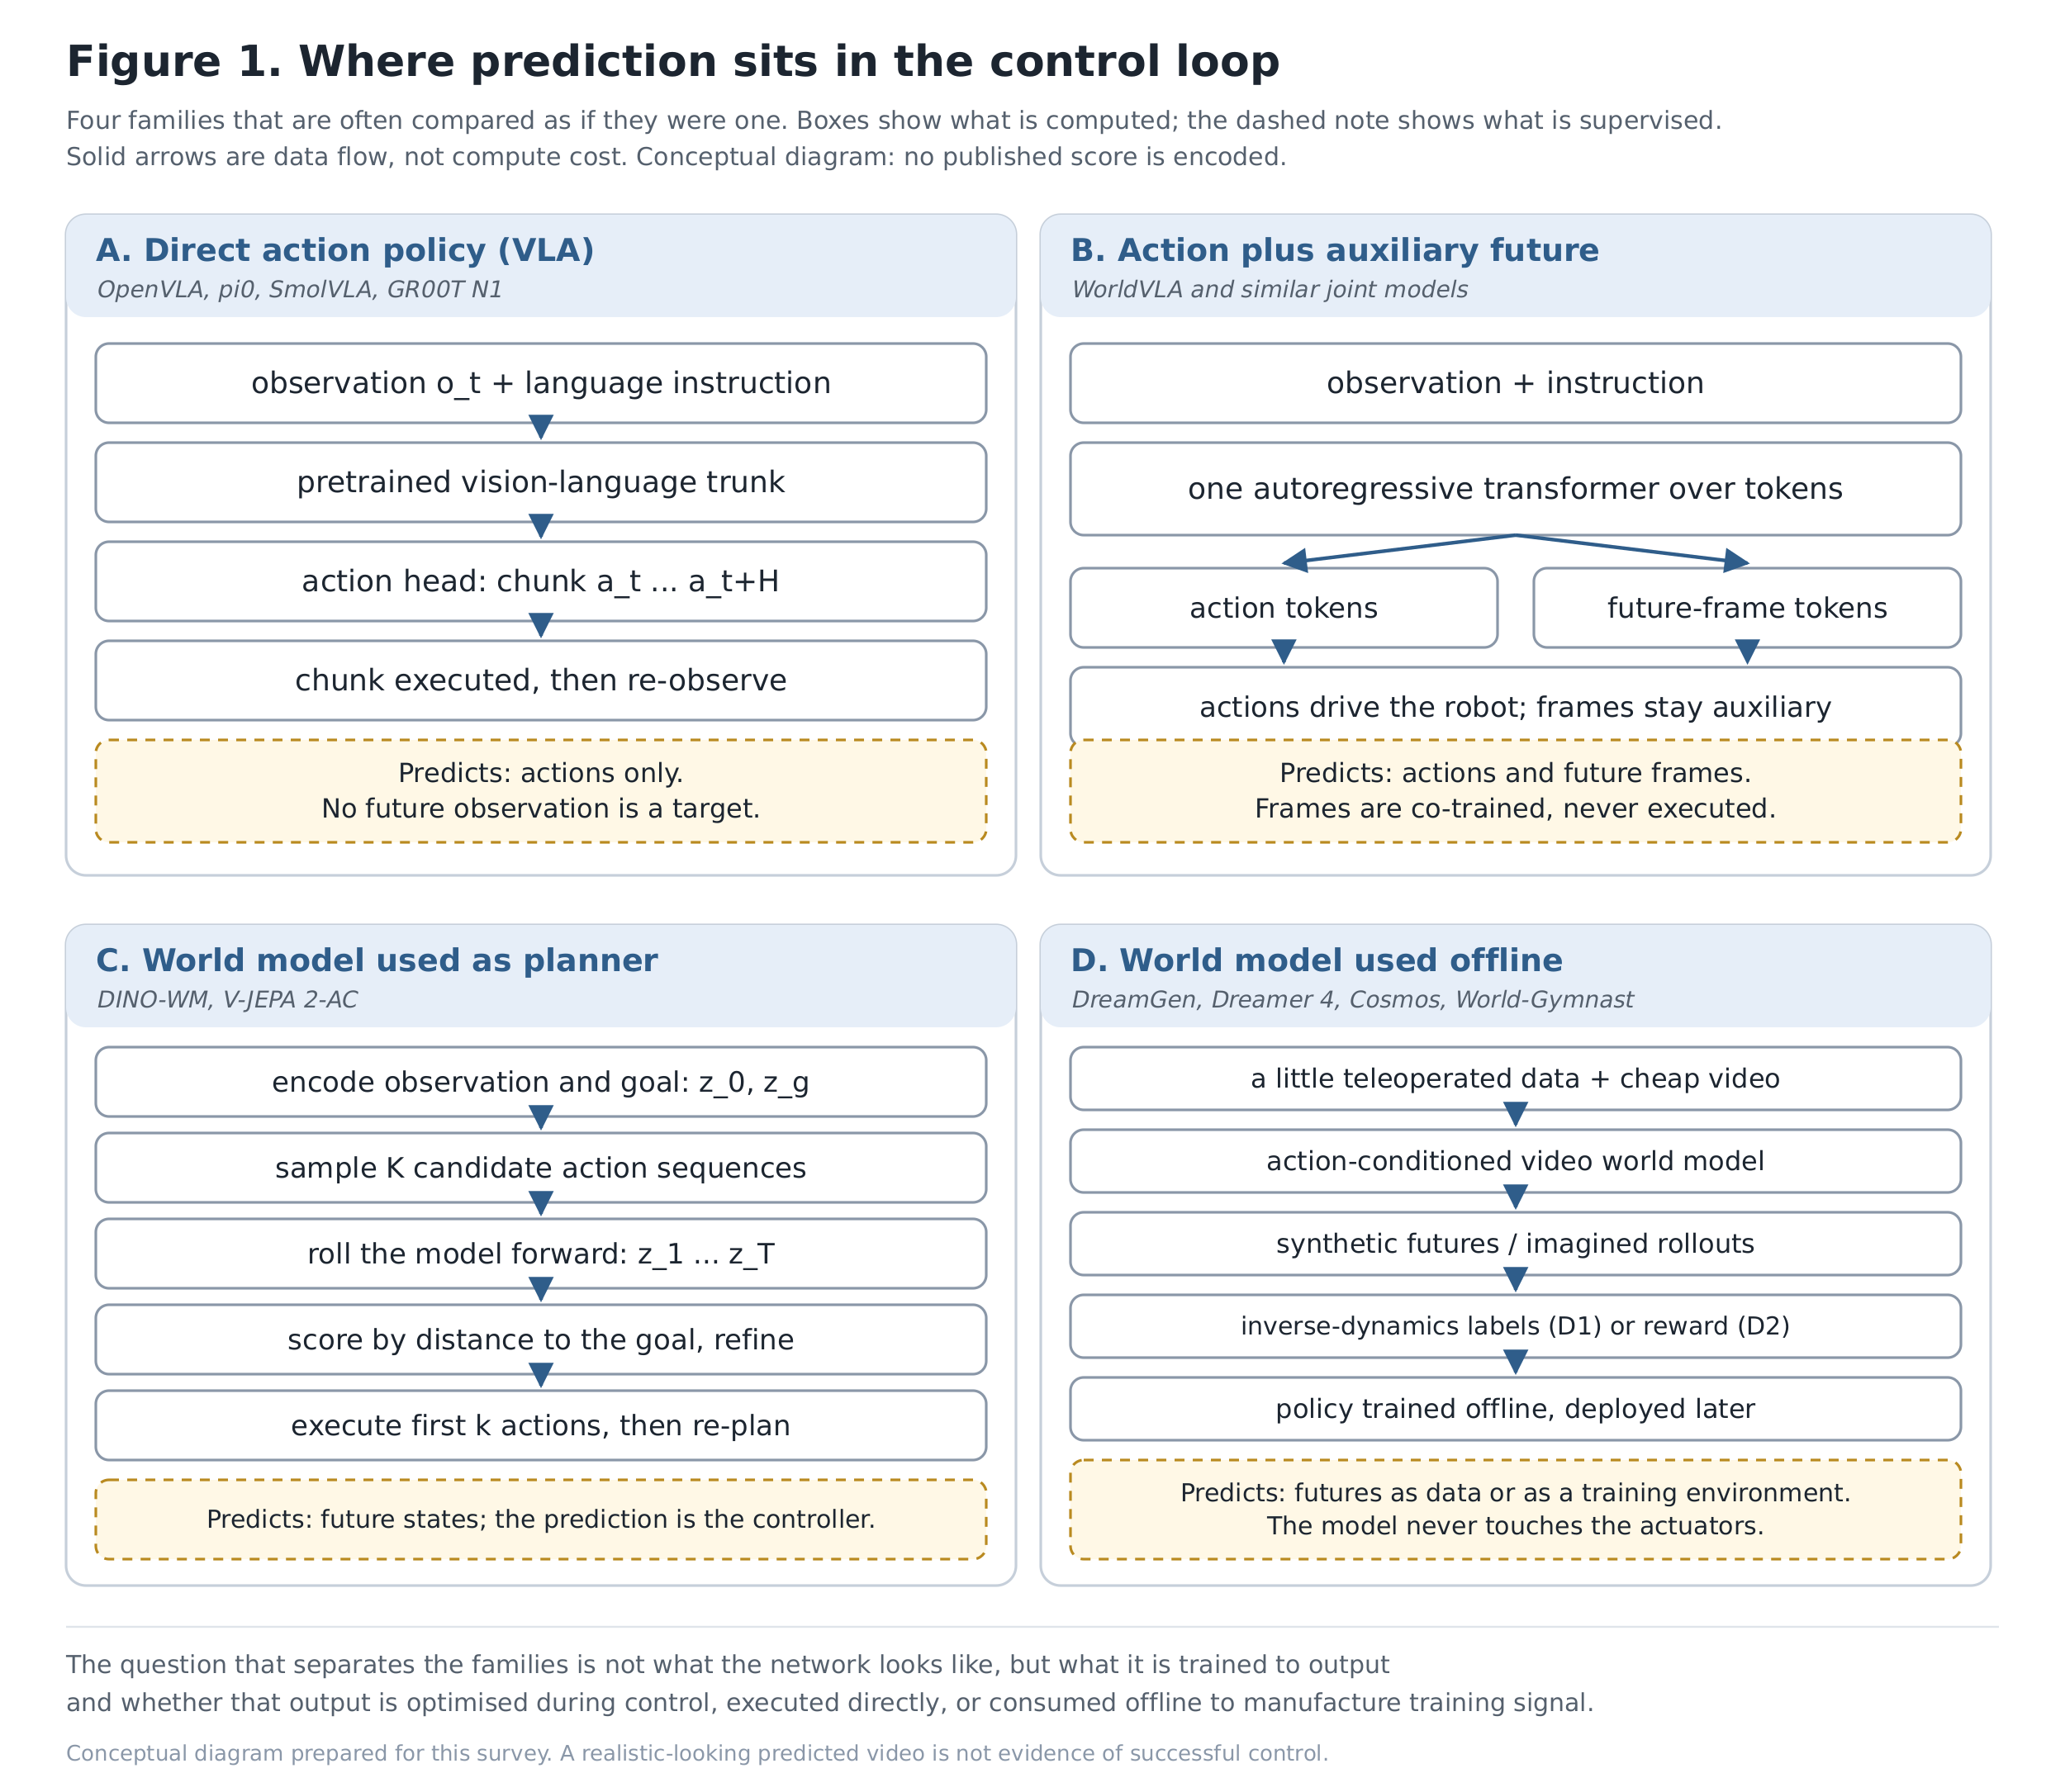
\includegraphics[width=1\textwidth,height=\textheight]{figures/fig1_prediction_in_loop.png}
\caption{Where prediction sits in the control loop. Four families are
drawn as data flow; the dashed note in each panel states what is
supervised. The diagram is conceptual and encodes no published score.}
\end{figure}

Comparable, with care:

\begin{itemize}
\tightlist
\item
  Same model, one factor changed. WorldVLA against its own action-only
  ablation is a legitimate comparison, because the data, architecture
  and evaluation are held fixed \citep{worldvla}. Ablations of this kind
  are the only place where ``prediction helps'' is a controlled claim.
\item
  Same benchmark, same protocol. LIBERO numbers from different papers
  are often quoted side by side. They are only comparable when the
  suite, the observation set, the action space and the number of
  demonstrations match; the benchmark's own paper documents how much
  those choices matter \citep{libero}.
\item
  Rankings, not scores. RoboArena's contribution is precisely that
  pairwise preferences aggregate more reliably than absolute success
  rates across heterogeneous policies \citep{roboarena}.
\end{itemize}

Not comparable, although frequently compared:

\begin{itemize}
\tightlist
\item
  Absolute success rates across embodiments. A humanoid task set and a
  table-top arm task set do not share a difficulty scale, and the
  denominators differ.
\item
  Simulation against real. A LIBERO score of one family and a real-arm
  score of another are two different measurements of two different
  systems; the gap between them is the sim-to-real problem, not a
  property of a method.
\item
  Predicted-video quality against control success. FVD and similar
  metrics measure distributional similarity of generated frames, and no
  paper in this corpus establishes a monotone relation between them and
  task success. A convincing rollout video is therefore an illustration,
  never a control result.
\item
  Data-efficiency claims expressed in ``times fewer samples'', because
  the baselines and the counting units differ between studies
  \citep{lbm, dino_wm}.
\end{itemize}

\begin{figure}
\centering
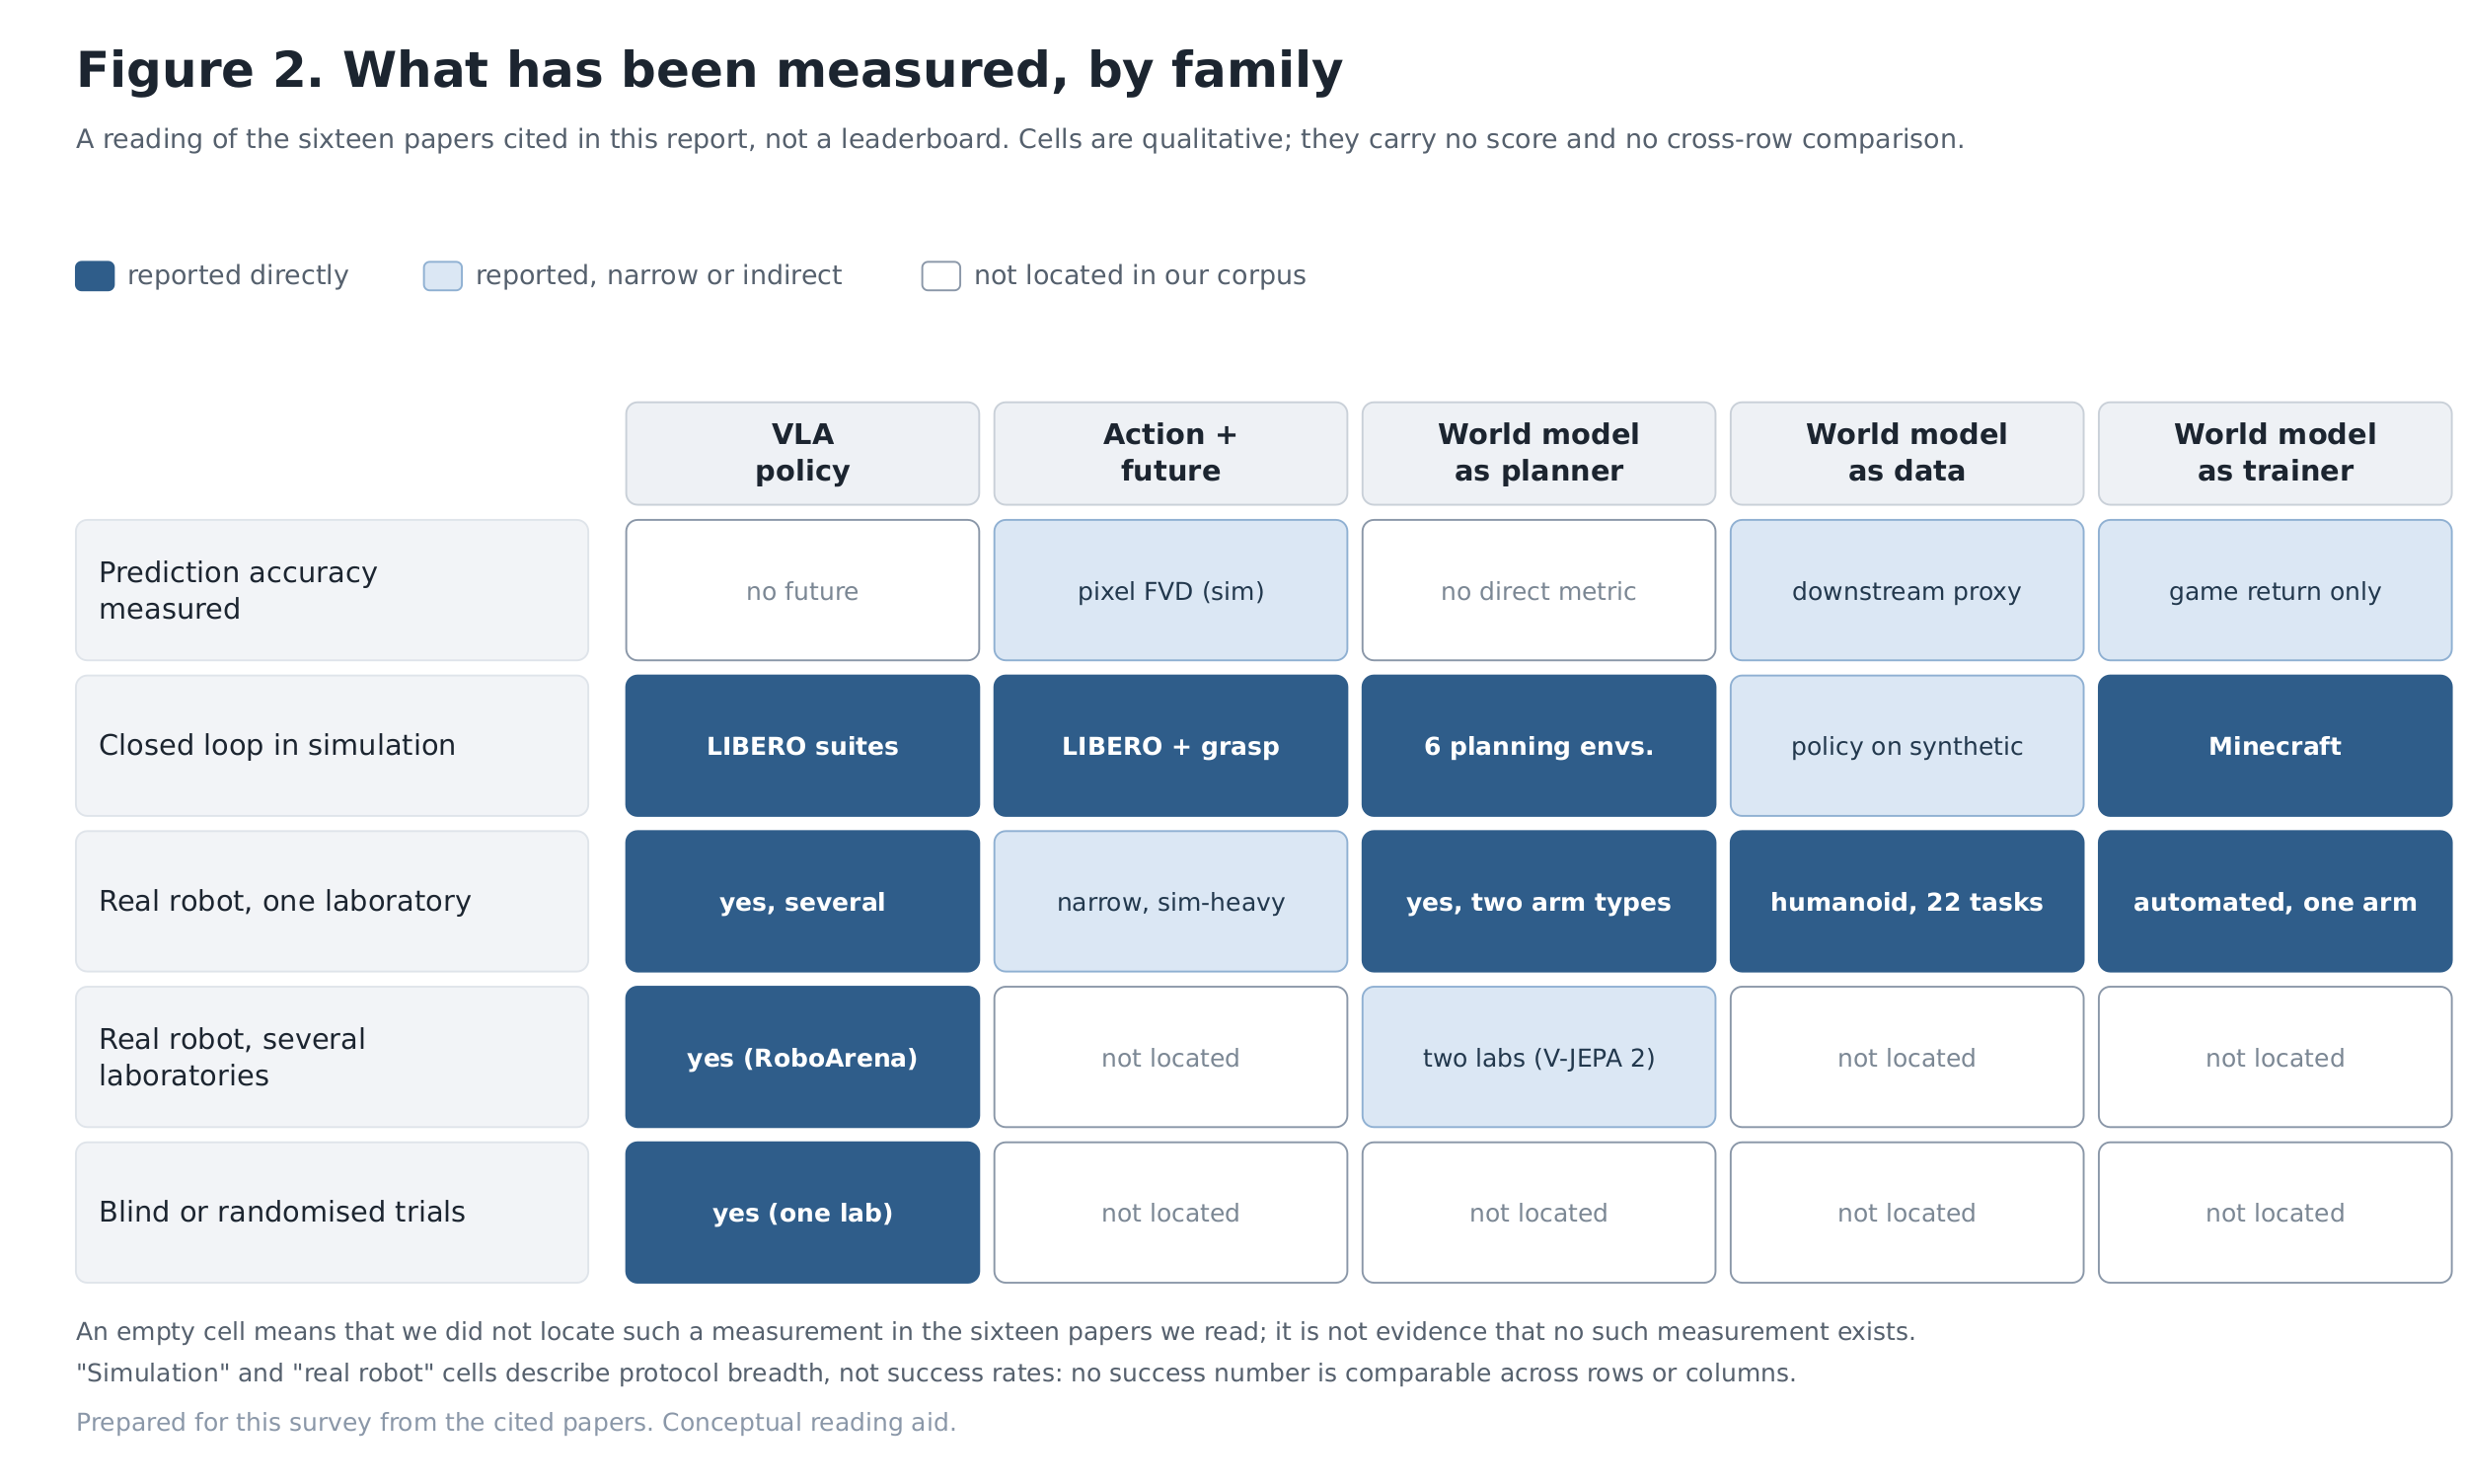
\includegraphics[width=1\textwidth,height=\textheight]{figures/fig2_evidence_map.png}
\caption{A coarse evidence map over the sixteen papers. Cells record
whether a measurement type was reported and how broad the protocol was;
they carry no score. ``Not located'' means absent from this corpus, not
absent from the literature.}
\end{figure}

Figure 2 makes the resulting shape visible. Only the direct-policy
column contains multi-institution evaluation at the level of a whole
study, where several groups run one shared protocol and the results can
be pooled: RoboArena's distributed arena and the blind comparison of
large behaviour models \citep{roboarena, lbm}. The planner column is not
uniformly single-site either: V-JEPA 2's action-conditioned planner was
demonstrated on two robot arms in two laboratories \citep{vjepa2}. That
is a two-laboratory demonstration of one system, which is weaker than a
shared protocol that many groups can use to rank arbitrary policies, but
it is more than a single-site result and it is recorded as such. The
trainer column's closed-loop evidence is single-site, and in both the
planner and trainer columns much of the supporting evidence is in
simulation or in a game. This is the single most important asymmetry for
a reader deciding where to spend effort, and it is a statement about
evaluation breadth, not about which model is smarter.

\hypertarget{code-simulation-and-data-resources-that-a-small-group-can-actually-use}{%
\subsection{10. Code, simulation and data resources that a small group
can actually
use}\label{code-simulation-and-data-resources-that-a-small-group-can-actually-use}}

Open weights and training code are available for OpenVLA, SmolVLA, GR00T
N1, V-JEPA 2 and Cosmos; DINO-WM and Dreamer 4 publish research code;
WorldVLA announces code alongside its paper
\citep{openvla, smolvla, groot_n1, vjepa2, cosmos, dino_wm, dreamer4, worldvla}.
pi-0 releases weights but not a full replication recipe \citep{pi0};
Gemini Robotics 1.5 releases neither \citep{gemini_robotics15};
World-Gymnast had no public artefacts at the time of writing
\citep{world_gymnast}. Licences differ, and Cosmos in particular carries
a use policy rather than an ordinary open-source licence, which matters
if the output is to be redistributed \citep{cosmos}.

For simulation, LIBERO is the workhorse for language-conditioned
manipulation and is used by most of the policy papers discussed here
\citep{libero}. It is not a physics-fidelity benchmark: it is a
task-diversity benchmark, and results in it saturate, which is why the
more recent papers add real-robot confirmation rather than higher
simulated scores.

\hypertarget{feasible-next-investigations-without-a-fleet}{%
\subsection{11. Feasible next investigations without a
fleet}\label{feasible-next-investigations-without-a-fleet}}

The following are ordered by cost, and each is designed so that a
negative result is still publishable inside a group.

\textbf{P1. Reproduce one action-only baseline and one auxiliary-future
variant on a single GPU.} Take an open VLA checkpoint, fine-tune it on a
small LIBERO suite, then add a next-frame prediction loss and re-run.
The question is whether the reported auxiliary-prediction gain survives
a different base model \citep{worldvla, libero}. Cost: GPU hours, no
hardware.

\textbf{P2. Measure whether world-model fidelity predicts planning
success.} Train a latent dynamics model on an offline dataset, then plot
planning success against held-out latent-prediction error as data scale
increases. This tests the assumption that better models make better
planners, which the literature asserts more often than it measures
\citep{dino_wm, vjepa2}. Cost: single GPU, public video.

\textbf{P3. Audit environment leakage in a published world-model
result.} For a paper that reports generalisation, take its pretraining
corpus and test whether the held-out scenes are visually retrievable
from it. This is a cheap, high-value check that no paper in this corpus
performs systematically \citep{world_gymnast, dreamgen}.

\textbf{P4. Compare planning against behaviour cloning under an equal
data budget.} Same offline data, same embodiment, one planner and one
direct policy, both evaluated on the same held-out tasks with a blind
scoring script. This is the comparison the field lacks and the one that
decides the practical question in Section 1.

\textbf{P5. Replicate a multi-site protocol at small scale.} RoboArena's
lesson is that pairwise preferences aggregate better than absolute
scores; a two-lab or two-operator version with a shared task list and a
fixed comparison budget is within reach of a small consortium and
directly addresses the weakest part of Figure 2 \citep{roboarena, lbm}.

\hypertarget{limitations-of-this-report}{%
\subsection{12. Limitations of this
report}\label{limitations-of-this-report}}

The corpus is sixteen papers, weighted towards 2024--2025, with a
two-paper 2026 slice; it is not a current or comprehensive survey of the
field, and it was assembled opportunistically rather than by a
registered protocol. Of those two 2026 items, one (World-Gymnast) was
read as a complete text, while the other (PlayWorld) is retained in the
evidence bundle as a substantial full-text HTML acquisition from which
this report used only abstract-level statements; what was acquired for
that paper therefore exceeds what this report actually read and relies
on. No number here was re-measured, no implementation was run, and no
benchmark was re-scored, so every quantitative statement is an
attributed claim under the original authors' conditions. Figures 1 and 2
are qualitative reading aids constructed for this report: they encode no
score, and their ``not located'' cells record the limits of this corpus.
The accompanying PDF was produced mechanically from this Markdown.
Figure layout is enforced geometrically in the figure generator, which
aborts on any text overflow. The rendered figures and two PDF pages were
inspected once with a vision model, whose only finding was duplicated
figure-caption prefixes, since corrected; a later re-inspection attempt
failed with a provider error and was not retried, so there has been no
automated page-by-page visual sign-off of every page of the final PDF,
and any such inspection would be a layout check rather than a scientific
review of the content.

\hypertarget{recommendation}{%
\subsection{13. Recommendation}\label{recommendation}}

Build on a direct action policy first. It has the shortest path from
public weights to a working system, it is where the evaluation
methodology is most mature, and its failure modes are the ones a new
group needs to learn to measure. Add prediction where it is cheap and
testable: an auxiliary future-prediction loss costs one extra decoder
and one ablation, and that is the experiment that tells you whether
prediction helps \emph{your} data. Treat world models as planners or
trainers only once an offline data pipeline and a scoring harness exist,
because both uses multiply the cost of every mistake in the data
pipeline. And when reading the next wave of results, ask the question
that separates the families: not how good the generated future looks,
but what was measured, on how many sites, with what protocol.

  \bibliography{references.bib}

\end{document}
